
\documentclass{beamer}


\usetheme{Madrid}
\usepackage{amsmath}

\title{Intro to AI and ML}

% A subtitle is optional and this may be deleted
\subtitle{Matrix Project}

\author{S Suprabath Reddy \and Srujan Kumar Bazar}


\date{14th February, 2019}

\AtBeginSubsection[]
{
  \begin{frame}<beamer>{Outline}
    \tableofcontents[currentsection,currentsubsection]
  \end{frame}
}

% Let's get started
\begin{document}

\begin{frame}
  \titlepage
\end{frame}


\begin{frame}{Question}
Two sides of a rhombus are along the lines, x - y + 1= 0 and 7x - y - 5 =0. If its diagonals intersect at (-1,-2), then find all its vertices.
  \newline
  \newline
JEE Mains 2016, Q.No - 31, Code-F
\end{frame}

\begin{frame}{Question in Matrix form}

Two sides of a rhombus are along the lines
\\
$ \begin{bmatrix}
  \ 1 &
  \ -1 \\
\end{bmatrix}
\textbf{x} + 1 = 0 $ 
\\ 
$  \begin{bmatrix}
  \ 7 &  
  \ -1 \\
\end{bmatrix} \textbf{x} - 5 = 0 $
\\
If its diagonals intersect at
$ 
\begin{bmatrix}
  \ -1 \\
  \ -2 \\
\end{bmatrix}
$
, then find all its vertices.\\
\end{frame}

\begin{frame}{Solution}
We have equations of two lines in matrix form. We can find one vertex by finding point of intersection of both the lines.
\newline
\newline
Vertex \textbf{A} from intersection of lines \textbf{L1} and\textbf{ L2}.
\newline
n_1 = 
$ 
\begin{bmatrix}
  \ 1 \\
  \ -1 \\
\end{bmatrix}
$ \hspace{20}
and  \hspace{20}
n_2 = 
$ 
\begin{bmatrix}
  \ 7 \\
  \ -1 \\
\end{bmatrix}
$
\newline
\ N^T = 
$ 
\begin{bmatrix}
  \ 1 & -1 \\
  \ 7 & -1 \\
\end{bmatrix}
$ \hspace{20}
and  \hspace{20} |N^{T}| = 6
\newline
N^{-T} = 
$ 
\begin{bmatrix}
  \ -1/6 & 1/6 \\
  \ -7/6 & 1/6 \\
\end{bmatrix}
$
\newline
p = 
$ 
\begin{bmatrix}
  \ -1 \\
  \ 5 \\
\end{bmatrix}
$ 

\textbf{A} = N^{-T}p = 
$ 
\begin{bmatrix}
  \ 1 \\
  \ 2 \\
\end{bmatrix}
$ 
\end{frame}

\begin{frame}{Solution}
Also given, mid-point O = 
$ 
\begin{bmatrix}
  \ -1 \\
  \ -2 \\
\end{bmatrix}
$ 
\newline
Since we have \textbf{A} and \textbf{O}, we can find opposite vertex of A which is \textbf{C}.
\newline
\textbf{C} = 2*O - A = 
$ 
\begin{bmatrix}
  \ -3 \\
  \ -6 \\
\end{bmatrix}
$ 
\newline
We know that diagonals of rhombus are perpendicular to each other. So, director vector of \textbf{AC} is normal vector of \textbf{BD}.
\newline
n = A - C = 
$ 
\begin{bmatrix}
  \ 4 \\
  \ 8 \\
\end{bmatrix}
$ 
\newline
We can find equation of BD using mid-point O.
\newline
p = (n.T)O = -20
\newline
BD:
$ \begin{bmatrix}
  \ 4 &
  \ 8 \\
\end{bmatrix}
\textbf{x} + 20 = 0 $ 
\newline
We can find other two vertices B and D using point of intersection of lines \textbf{AB,BD} and \textbf{AD,BD} respectively like we did between L1 and L2.
\newline
\textbf{B} = 
$ 
\begin{bmatrix}
  \ -7/3 \\
  \ -4/3 \\
\end{bmatrix}
$ \hspace{20}
and  \hspace{20}
\textbf{D} = 
$ 
\begin{bmatrix}
  \ 1/3 \\
  \ -8/3 \\
\end{bmatrix}
$

\end{frame}

\begin{frame}{Graph}
\centering
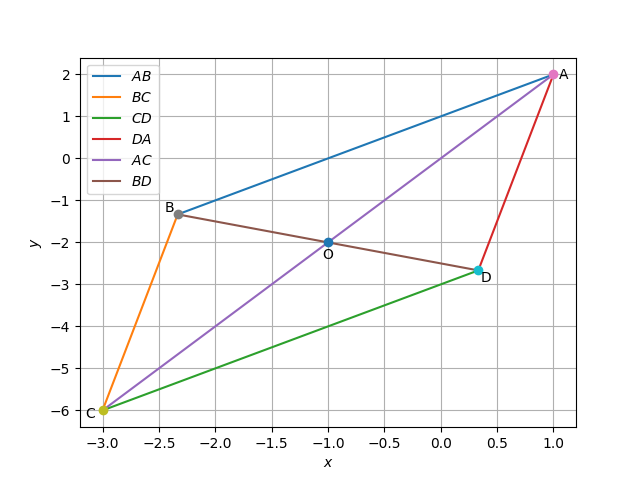
\includegraphics[scale=0.7]{Figure_1.png}
\end{frame}

\end{document}


